\chapter{Mesures du comportement du système sans le filtre coupe-bande}
\label{annexe:SansNotch}
Cette annexe présente la mesure du système en fonctionnement, avec le filtre coupe-bande retiré de la régulation.

Le comportement du pompage, du tangage et du roulis est d'abord présenté de la \autoref{fig:PompageSansNotch} à la \autoref{fig:RoulisSansNotch} :

\begin{figure}[H]
    \centering
    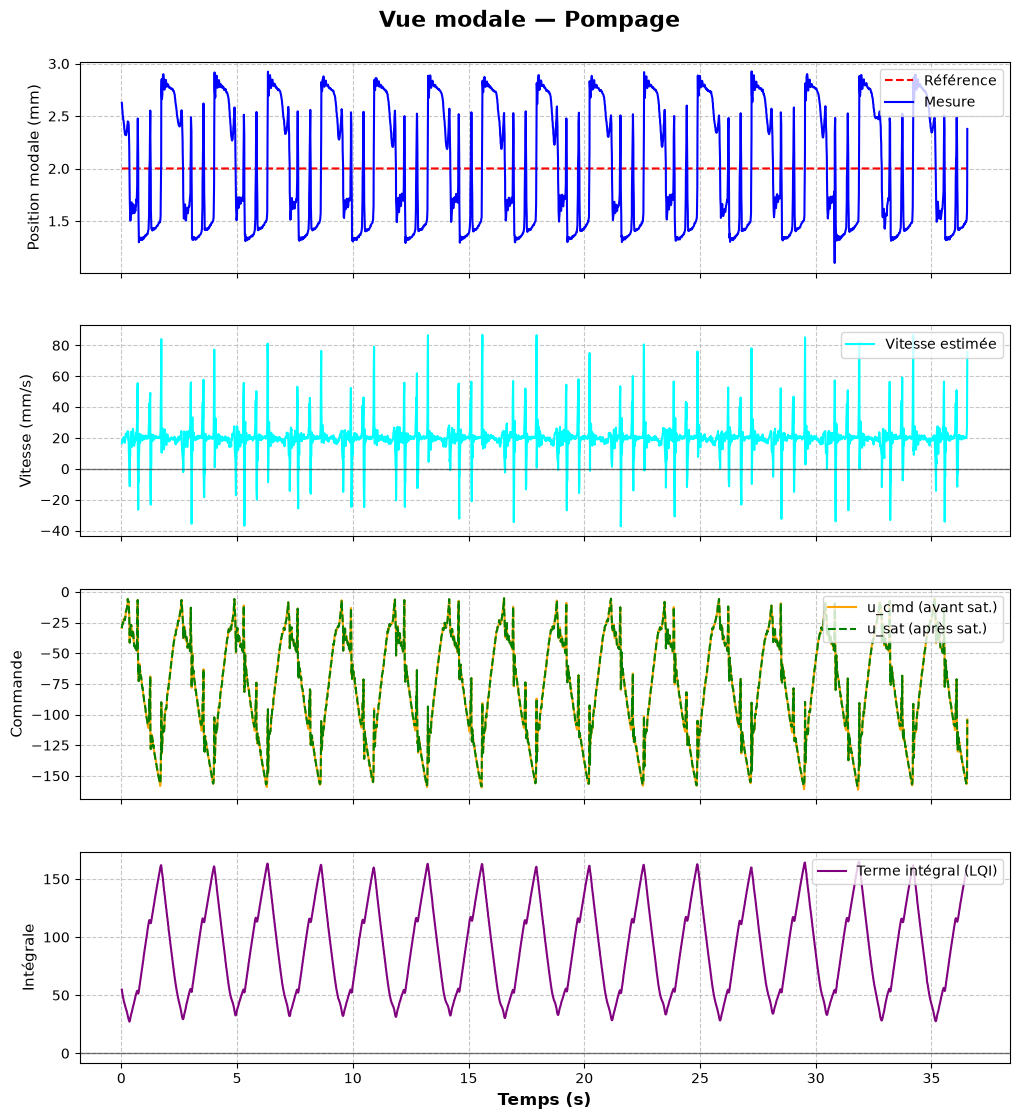
\includegraphics[width=1\linewidth]{assets/appendix/13-MesureSansFiltre/pompage.png}
    \caption{Mesure du pompage (Z) sans le filtre coupe-bande}
    \label{fig:PompageSansNotch}
\end{figure}

\begin{figure}[H]
    \centering
    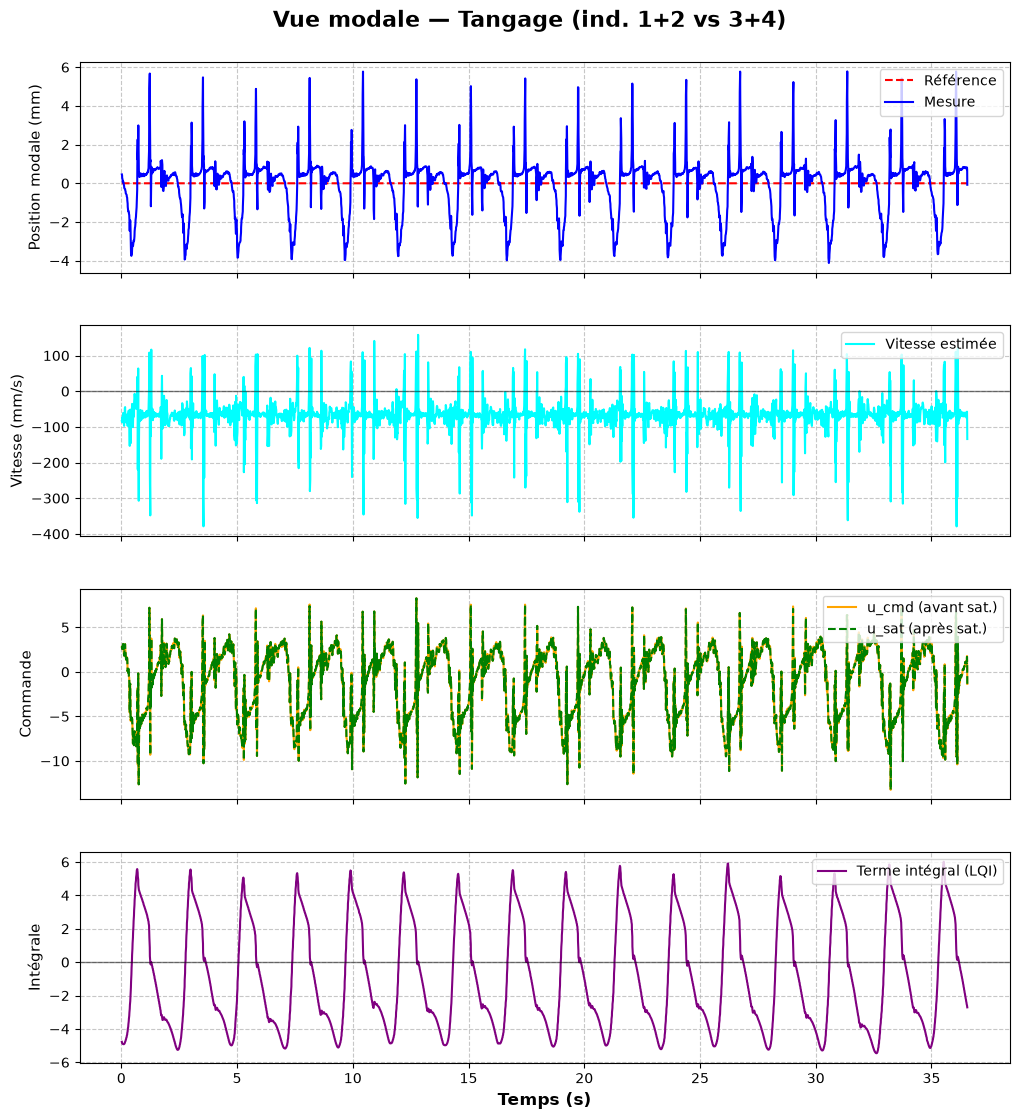
\includegraphics[width=1\linewidth]{assets/appendix/13-MesureSansFiltre/tangage.png}
    \caption{Mesure du tangage ($\theta$) sans le filtre coupe-bande}
    \label{fig:TangageSansNotch}
\end{figure}

\begin{figure}[H]
    \centering
    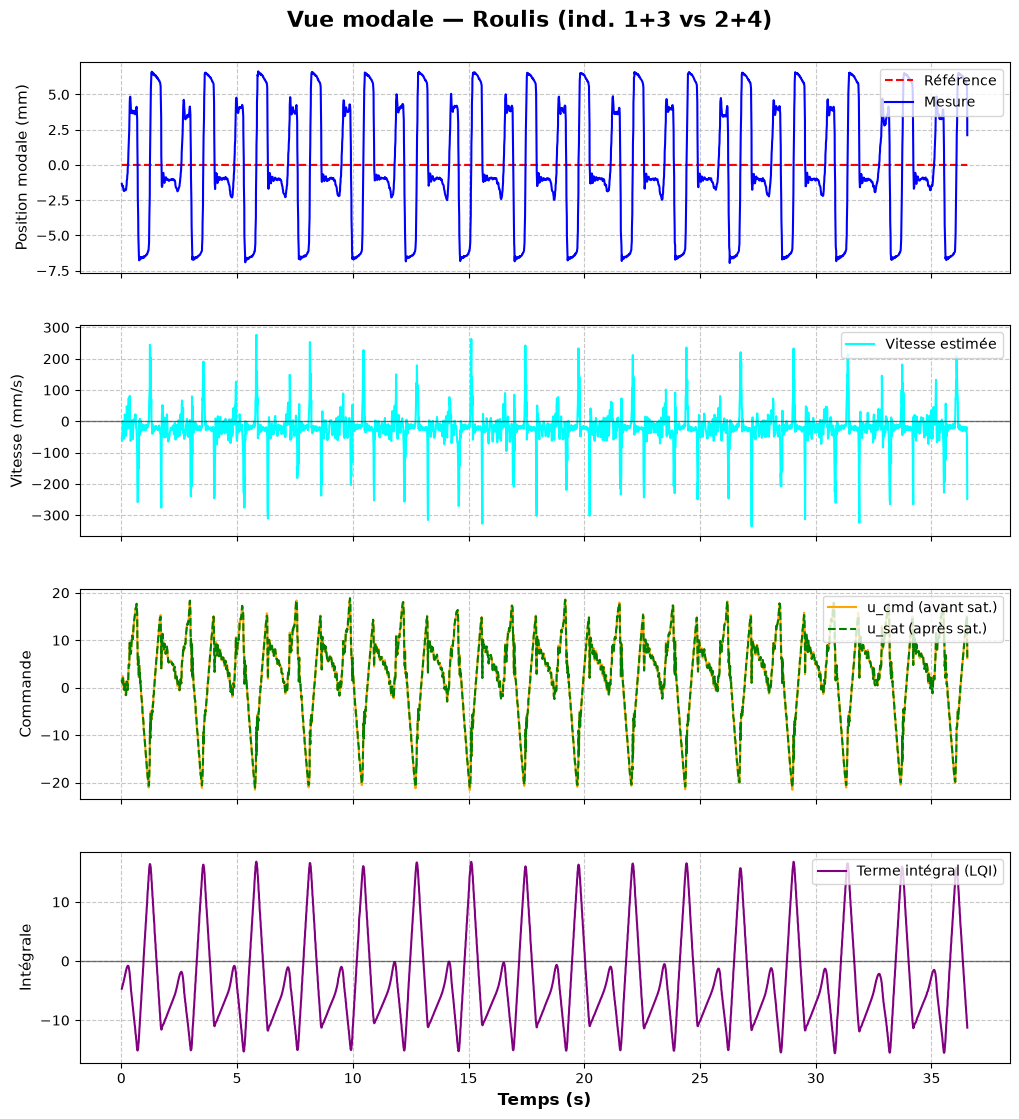
\includegraphics[width=1\linewidth]{assets/appendix/13-MesureSansFiltre/roulis.png}
    \caption{Mesure du roulis ($\varphi$) sans le filtre coupe-bande}
    \label{fig:RoulisSansNotch}
\end{figure}

Le comportement par inducteur est ensuite représenté de la \autoref{fig:Ind1SansNotch} à la \autoref{fig:Ind4SansNotch} :

\begin{figure}[H]
    \centering
    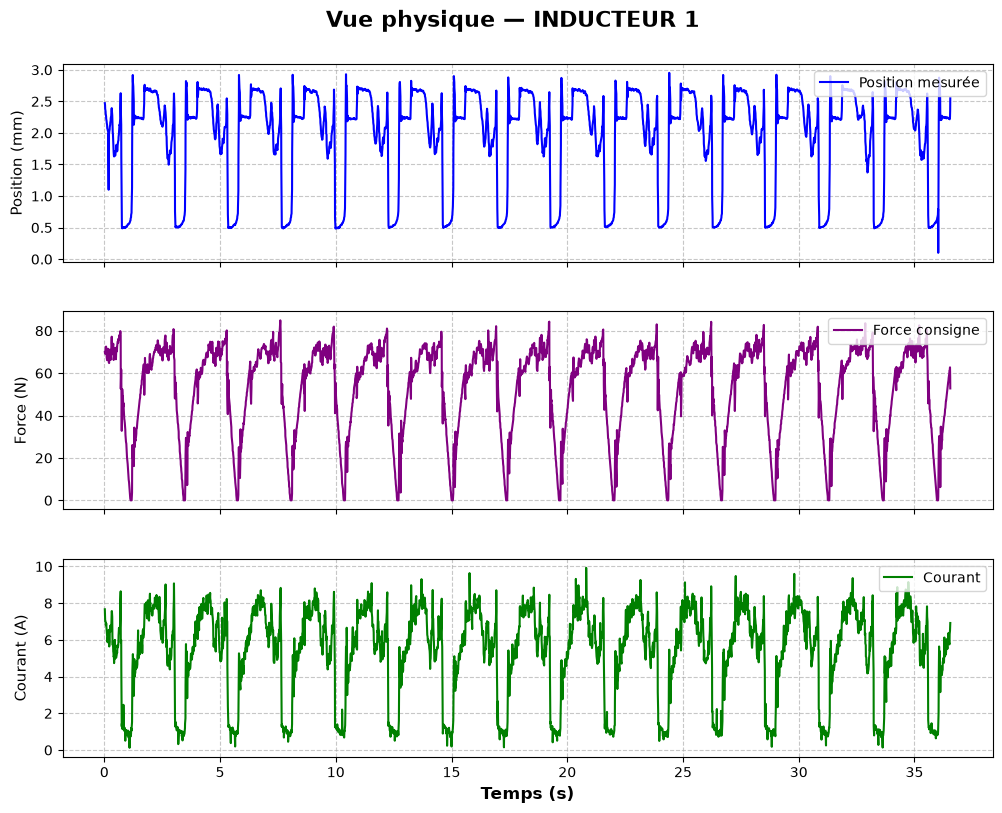
\includegraphics[width=1\linewidth]{assets/appendix/13-MesureSansFiltre/Ind1.png}
    \caption{Mesure du comportement de l'inducteur 1 sans le filtre coupe-bande}
    \label{fig:Ind1SansNotch}
\end{figure}

\begin{figure}[H]
    \centering
    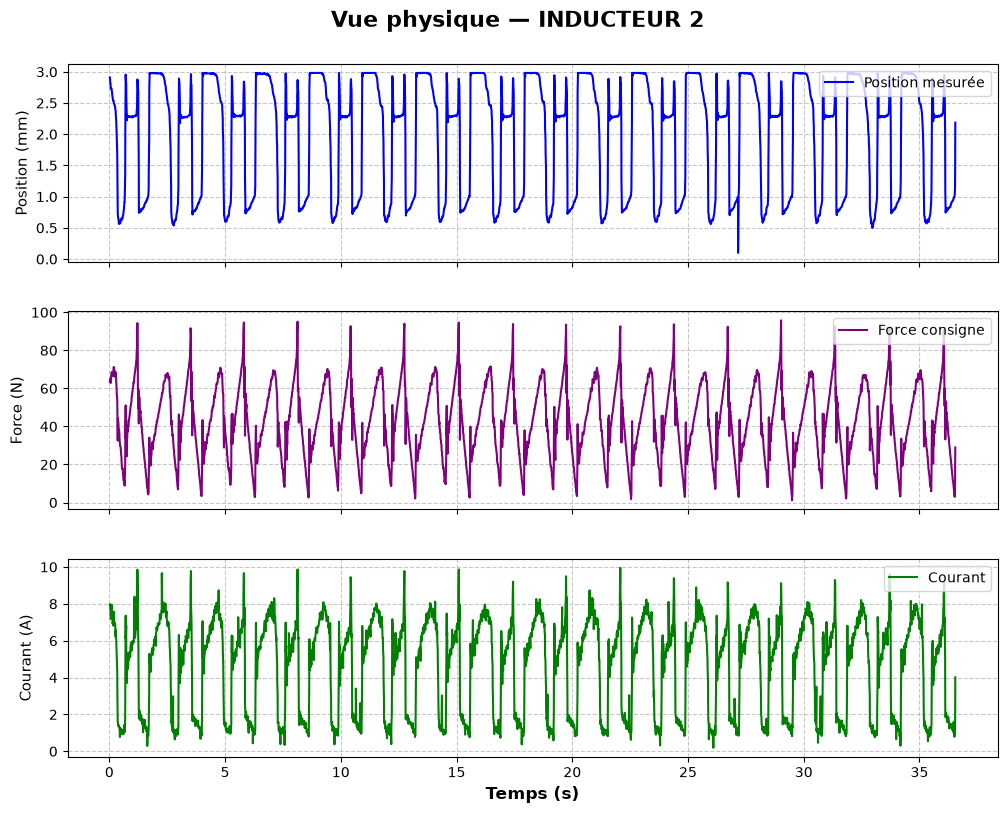
\includegraphics[width=1\linewidth]{assets/appendix/13-MesureSansFiltre/Ind2.png}
    \caption{Mesure du comportement de l'inducteur 2 sans le filtre coupe-bande}
    \label{fig:Ind2SansNotch}
\end{figure}

\begin{figure}[H]
    \centering
    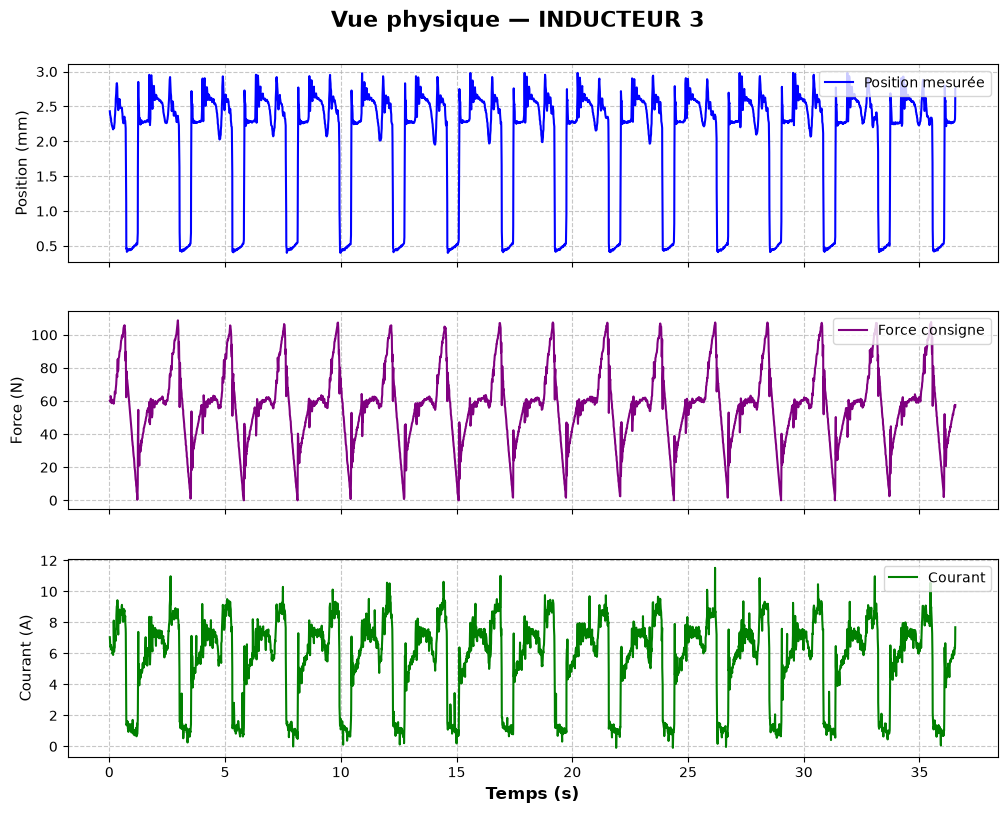
\includegraphics[width=1\linewidth]{assets/appendix/13-MesureSansFiltre/Ind3.png}
    \caption{Mesure du comportement de l'inducteur 3 sans le filtre coupe-bande}
    \label{fig:Ind3SansNotch}
\end{figure}

\begin{figure}[H]
    \centering
    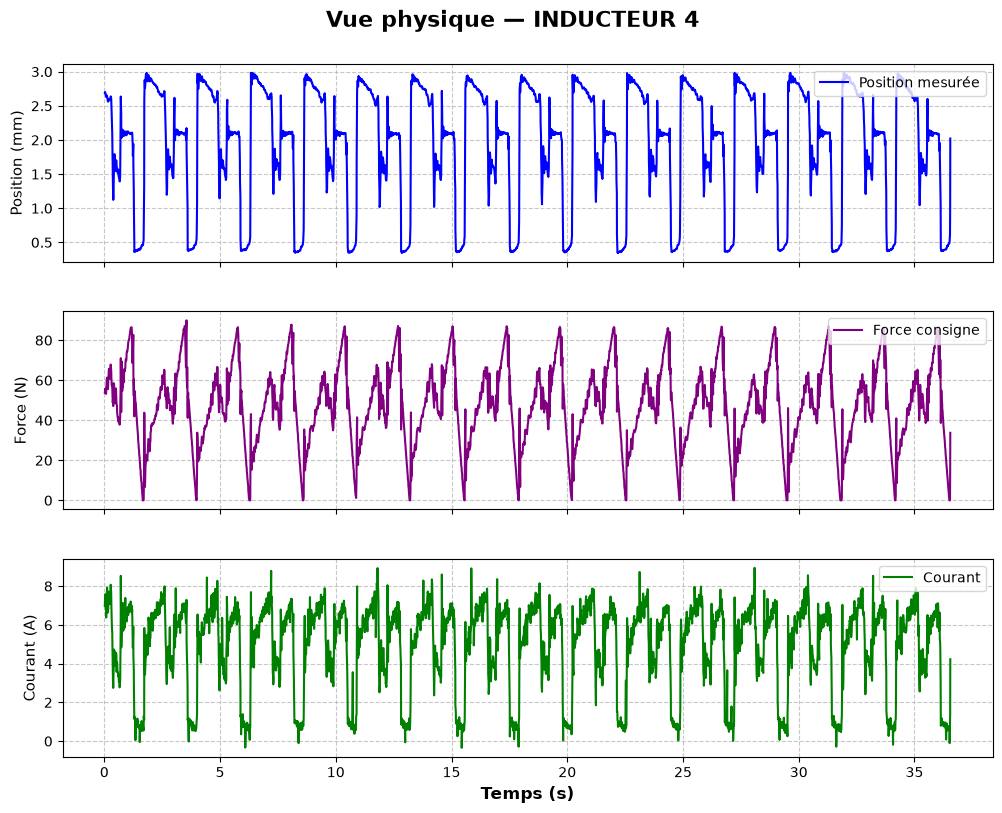
\includegraphics[width=1\linewidth]{assets/appendix/13-MesureSansFiltre/Ind4.png}
    \caption{Mesure du comportement de l'inducteur 4 sans le filtre coupe-bande}
    \label{fig:Ind4SansNotch}
\end{figure}

Ces mesures montrent une oscillation importante du système, ce qui confirme que le filtre coupe-bande est bel et bien nécessaire à la synthèse de la régulation de position.

Il serait cependant intéressant d'approfondir la recherche sur la raison de l'emploi de ce filtre, dont le rôle reste à ce jour associé à un comportement non expliqué.
